% !TeX spellcheck = en_US
\section{MBS System Model}
\label{sec:520_SystemModel}
The \ac{MBS} scenarios discussed in Section~\ref{sec:220_Scenario} are classified into remote, in situ, and hybrid streaming.
What the scenarios have in common is that they consist of at least one recording device transmitting video to a receiver, which can be either a smart mobile device or a remote server.
\subsection{Recording Device}
The recording device consists of two important components: the video recording \ac{API} and the recording buffer.
\subsubsection{Media Recording API}
Each \ac{MBS} has access to media capturing sensors. 
It is assumed that these sensors map potentially analog signals into digital data. 
This step requires the support of a video codec. 

A digital video stream is made available in an encoding step that ensures a suitable compression of the data, so that it is feasible to be streamed in today's mobile networks.
Typical encodings supported by smart mobile devices are H.264/\ac{AVC}~\cite{Wiegand2003} or H.265/\ac{HEVC}~\cite{Sullivan2012}.
An additional requirement is that available smartphones have the capability to encode and decode video in real-time.
This is possible if the devices posses a video codec circuit, which enables en- and decoding in hardware.
Today, such a hardware support is available for many devices when using H.264/\ac{AVC}~\cite{Wiegand2003}.
A final requirement describes that a video codec supports streaming - meaning that parts of a video can already be played without possessing the complete video.
This is essential for live streaming, but not supported by many video containers.
The non-encapsulated, raw H.264/\ac{AVC} and H.265/\ac{HEVC}, as well as the video container \ac{MPEG-TS}, support this requirement.
As a result, the media recording \ac{API} provides a streamable, compressed video stream to the recording buffer.
\subsubsection{Recording Buffer}
The recording buffer is the interface to the \ac{MBS}.
It is constantly filled with video from the media recording \ac{API} (see Figure~\ref{fig:520_videorecordingapi}) and read by the \ac{MBS}.
A circular buffer is used, which processes data in \ac{FIFO} order and does not consume more memory than the smart mobile device can offer.
The size of the video recording buffer is limited to $w_{SB}$ video chunks.
A filled buffer is overwritten in \ac{FIFO} order, resulting in the loss of to-be-transmitted video chunks.
Thus, each available chunk in the recording buffer must represent an independently decodable video segment.
\begin{figure}
\centering
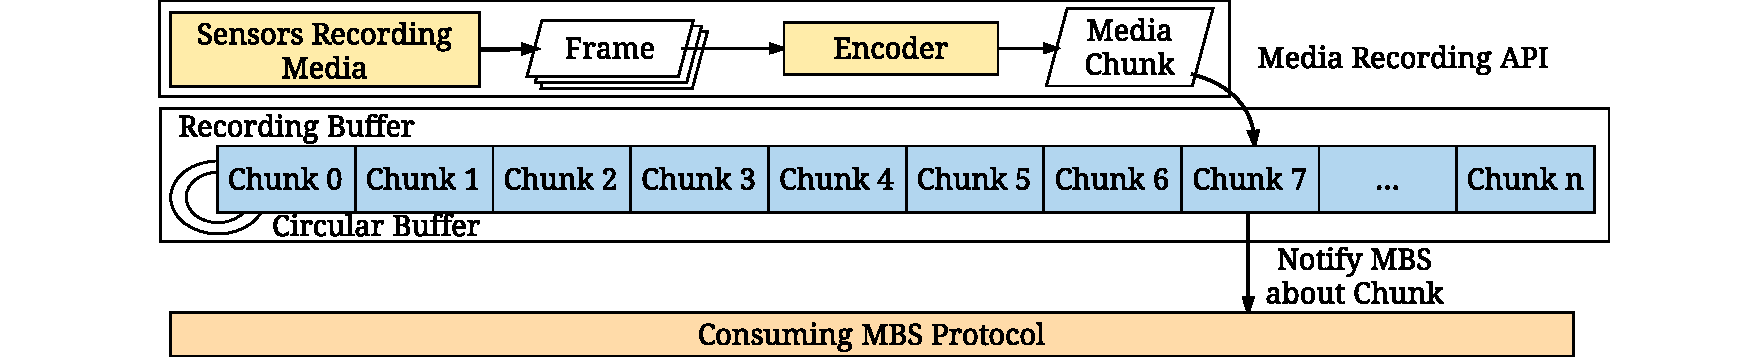
\includegraphics[width=\linewidth]{gfx/500_MobileUpload/MediaRecordingAPI}
\caption{Example of a Media Recording API and Recording Buffer.}
\label{fig:520_videorecordingapi}
\end{figure}

The media recording \ac{API} consecutively writes video chunks to the recording buffer, e.g., when recording a video frame.
As soon as a decodable chunk is available, the recording buffer informs the uploading mechanisms in the \ac{MBS} to transfer the video chunk. 
In most cases, this video chunk is passed instantly, but stored in the recording buffer in order to allow retransmission if a message is lost.
Thus, the buffer supports random access, which allows for up to the last $w_{SB}$ chunks to be retransmitted.
If the upload rate is below the bit rate of the recorded video, data can be consumed by the \ac{MBS} as soon as all preceding chunks are processed.
\subsection{Receiver}
Receivers of the video stream have a buffer for storing incoming video chunks.
It builds the abstraction to the higher layer application sink, which processes video chunks.
\subsubsection{Receiver Buffer}
Similar to the recording device, a buffer is assumed on the receiver side.
It stores video chunks until they are consumed by a multimedia application.
The receiver has a limited window of cached video chunks of size $w_{RB}$.
The processing is similar to the recording side in \ac{FIFO} order and uses a circular buffer.
In contrast to the video sending device, the receiver manages multiple buffers in relation to the number of actively streaming senders. 
All receiving buffers are available to the application sink and have to be kept in sync.
\subsubsection{Application Sink}
An application sink accesses a video buffer, and further processes the video. 
On the receiver side, applications consuming the video stream can be video players, video streaming servers, or sophisticated multimedia applications such as video composition systems.
Video players consume the video stream instantly by decoding and visualizing it on a display.
This is a common approach for the in situ streaming scenario as discussed in Section~\ref{sec:520_scenario_insitu}.
The video stream can also be received by a video streaming server, which ingests it into a distribution network for remote receiving and playback.
As an example for a multimedia application, a video composition system is discussed in Chapter~\ref{chapter:600_videocomposition} and in the previous chapter describing the \ac{PaSC}.
\subsection{Further Assumptions for the System Model}
It is important to know that modeling of lower layer protocols is not part of this thesis - as it focuses on the \ac{MBS} design on the application layer of the \ac{ISO}/\ac{OSI} model.
Furthermore, standard protocols are used on the transport layer, i.e., \ac{TCP} and \ac{UDP}.
No modifications on the lower layers are required.
It is assumed that the functionality is managed by an \ac{OS} and can be accessed by standard Berkeley sockets~\cite{ISOIECIEEEStandard99452009}.
%  -  -  -  -  -  -  -  -  -  -  -  -  -  -  -  -  -  -  -  -  -  - --
\section{Study on Adaptations in MBSes}
\label{sec:520_design_intro}
In a study of the advantages and disadvantages of different \ac{MBS}s, mechanisms and concepts are identified which should be supported by \ac{LiViU}. 
The study is performed in a simulation environment, allowing for a large-scale analysis of the potential for adaptation. 
\subsection{Video Upload Protocols}
\label{sec:520_design_upload_mechanisms}
Five upload protocols, including industry standards and research proposals, are investigated for their use in an adaptive manner. The focus lies on the leveraged transport mechanisms, scheduling of video chunks, and coordination of streaming session participants. 
Aspects such as security, encryption, and \ac{DRM} are out of the scope of this thesis.
\subsubsection{\acf{RTMP}}
The first protocol investigated is the de-facto standard for \ac{MBS}, as they are used by the major platforms YouNow, Twitch.tv, Periscope, YouTube.Live and Facebook.Live.
A detailed discussion of \ac{RTMP} is given in Section~\ref{sec:220_existing_mbs}.
For the classification of the protocol, it is important to know that it uses \ac{TCP} as the transport layer protocol and relies on a push-based delivery of media chunks from the recording device.
\subsubsection{\acf{RTMFP}}
Derived from \ac{RTMP}, the \ac{RTMFP}~\cite{rfc7016} replaces the connection-oriented \ac{TCP} transport mechanism with the datagram-oriented \ac{UDP}.
Video streams are transmitted on top of a connection in flows that are pushed from a recording device to a receiver.
Similar to \ac{RTMP}, these media flows are message-based.
It provides a higher speed for connection restoring and \ac{IP} mobility support which is not supported by the connection-oriented \ac{TCP}. 
In contrast to the \ac{RTMP} design, \ac{RTMFP} has been designed for client-server as well as for \ac{P2P} systems.
Underlying the unidirectional flows are bi-directional connections, which are established in an initial handshake procedure.

\ac{RTMFP} is session-based and establishes the session in two round trips~\cite{rfc7016}. 
A sender initiates the session by sending a single \emph{IHello} ("Initiator Hello") message.
The response contains a cookie, which allows the second round trip and final session establishment, known as keying.
Another send-and-response round establishes an optionally encrypted video session.
After the response is received, the initial video chunks can be exchanged.
The behavior for session establishment is quite similar to the procedure of \ac{RTMP}, but \ac{RTMFP} has to handle message losses in the application layer.

To ensure a reliable transmission over \ac{UDP}, \ac{RTMFP} assumes that the receiver acknowledges all messages.
\ac{RTMFP} implements a congestion control that needs to comply with Internet recommendations~\cite{rfc2914} and which is not allowed to be more aggressive than \ac{TCP}'s slow start algorithm.
The protocol requires application layer solutions for coping with packet losses and an in-order transmission of video chunks.
Due to the reduced overhead and latency of \ac{UDP}-based protocols, we assume that it is better suited for the live streaming applied in \ac{MBS}. 
\subsubsection{\acf{DASH-U}}
In recent years, \ac{HTTP}-based video streaming approaches have gained significant interest. 
The \ac{MPEG} \ac{DASH}~\cite{Stockhammer2011} standard defines network communication using \ac{HTTP} (\ac{TCP}) as well as the description of the video in a manifest, called the \ac{MPD}.
This pull-based video streaming scheme is used for the design of \ac{DASH-U}.
Using \ac{DASH} in an \ac{MBS} requires that the receiver requests video segments. 
These requests can regularly be planned, e.g., with a fixed frequency, or they can be event-based, e.g., after a \ac{DASH} segment is received.
Also, the video stream receiver can specify rules to request only specific video segments.
Each client transmits segments of a video only if they are requested by the receiver.
The underlying request-response (pull-based) communication pattern is very costly in terms of overhead.
On the other hand, the method is well-suited for scenarios where the receiver requires only a few video segments from each source. 
The control of what video stream is requested at which point in time lies at the server.
\subsubsection{\acf{DASH-P}}
Seo et al.~\cite{Seo2012} propose the \ac{DASH-P} as a prototypically evaluated upload protocol. 
As the name implies, communication in \ac{DASH-P} is based on the transmission of video segments via \ac{HTTP} POST requests, i.e., the device pushes video segments.
Whereas in \ac{DASH-U} the server requests individual segments using \ac{HTTP} GET requests, \ac{DASH-P} continuously pushes the video segments to the receiver. 
The overall delay until a segment is available on the streaming server is lower when the two approaches are compared.
An advantage of using \ac{HTTP} instead of a dedicated streaming protocol such as \ac{RTMP} is that no session or state has to be established before a new segment is transmitted.
\subsubsection{\acf{UDP-PL}}
The majority of the existing algorithms rely on \ac{TCP} as a transport mechanism.
\ac{UDP} has certain advantages when it comes to live video streaming, as the overhead and latency is lower in comparison to \ac{TCP}.
Pull- and \ac{UDP}-based streaming protocols are neither widely used nor standardized.
We propose a minimal video upload protocol which allows a client to inform a server about an available video stream.
The server immediately starts pulling available video segments over \ac{UDP}.
Also, only minimal modifications are made to compensate for the weaknesses of \ac{UDP}.
To allow for the compensation of transmission errors, an \ac{ARQ} concealment technique is implemented (see Section~\ref{sec:522_CopingUnreliabilityUDP}).
In comparison to \ac{RTMFP}, this protocol operates with pull-based scheduling and leverages only a minimal session management, i.e., no congestion control, and no encryption or state management.
\subsubsection{"Adaptive"}
Also, a protocol is implemented which encapsulates the protocols \ac{RTMP}, \ac{RTMFP}, \ac{DASH-U}, \ac{UDP-PL}, and \ac{DASH-P} to always select the best protocol for a given performance metric.
The performance metrics implemented and evaluated are described in Section~\ref{sec:520_metrics}.
An application can specify the performance metric and triggers the evaluation runs to determine the performance of each protocol.
If multiple metrics are defined and evaluated, this allows an application to switch the used performance metric at runtime.
The adaptive usage of the protocols is called "Adaptive". 
\paragraph{Extended System Model}
\label{sec:520_extendedSystemModel}
Derived from the system model described in Section~\ref{sec:520_SystemModel}, a component for coordinating and executing the adaptation between the different \ac{MBS}s is required.
On both the sender and the receiver side, buffers act as a decoupling feature from the application, i.e., the video recording \ac{API} or application sink consuming the video stream.
Buffered video chunks are accessed by the transmission layer which is an artificially introduced layer for all mechanisms of an \ac{MBS}.
The transmission layer allows the adaptation of scheduling schemes - either push- or pull-based streaming.
In this context, the transmission layer is only aware of the currently used transport protocol, which can either be \ac{UDP} or \ac{TCP}.
The concept of the transmission layer for the adaptive \ac{MBS} is depicted in Figure~\ref{fig:520_architecture_overview}.
\begin{figure}[tbh]
\centering
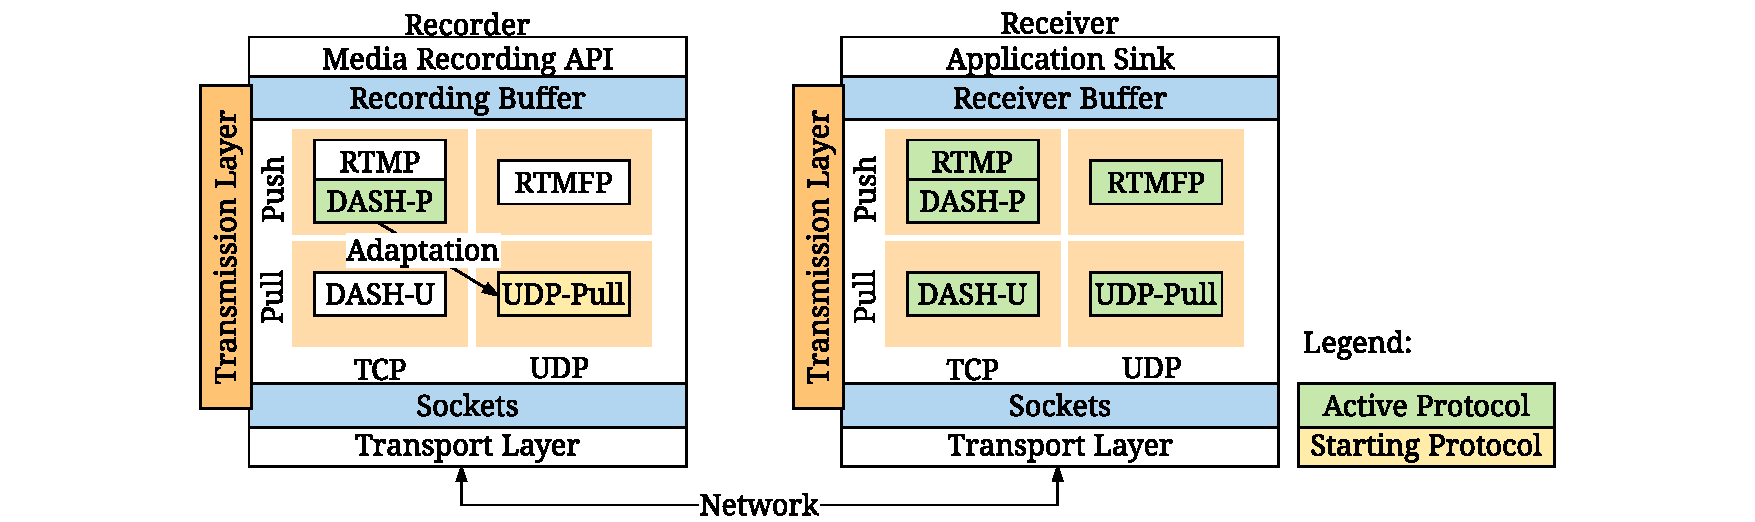
\includegraphics[width=\linewidth]{./gfx/500_MobileUpload/architecture_overview_embedded}
\caption[Concept on the transmission layer]{Concept of the transmission layer including the adaptation of \ac{MBS} upload protocols.}
\label{fig:520_architecture_overview}
\end{figure}

\paragraph{Contact Management}
Different upload protocols operate within the transmission layer.
They have in common that they have to manage their \emph{contacts}. To establish a transmission, the remote addresses are managed as so-called contacts. 
A contact is a remote device that participates in a streaming session, e.g., by receiving the stream. 
Contacts represent a unique combination of an \ac{IP} address and the port of the upload protocol. 
When run in parallel, different protocols are distinguished by the used network port address. 
Each protocol has its own, often standardized, port for communication.

\paragraph{Adapting between the Protocols}
"Adaptive" is configured to switch to a protocol which performs best for a given performance metric (Section~\ref{sec:520_metrics}).
A requirement is expressed as a performance metric, which can be measured during the runtime of a protocol.
Based on the result of a performance metric, "Adaptive" decides which protocol to choose. 
The measurement of the metrics and configuration of "Adaptive" to pursue differing requirements at different points in time is discussed in the simulative evaluation in Section~\ref{sec:520_metrics}.
\paragraph{Adaptive Video Streaming}
"Adaptive" includes the creation of multiple video representations with differing bit rates and their transmission to a receiver.
The concept of adaptive video streaming as a form of content adaption has been discussed in Section~\ref{sec:205_video_adaptation}.
For the discussion of \ac{MBS}, it is assumed that the recording device encodes $n$ video representations differing in the bit rate.
Each representation is encoded by an \ac{SVLC}, such as H.264/\ac{AVC} or H.265/\ac{HEVC}.
At any given moment, only one representation is chosen for transmission.
The selection is based on the measured application layer throughput rate for a device, so that the bit rate of a video must be below the available throughput rate.
\subsection{Assessing the Potential of Transitions between Upload Protocols}
\label{sec:520_simulativeAnalysis}
A simulative analysis of the proposed system model is conducted to understand which mechanisms of the upload protocols show superior performance under varying environmental conditions.
The findings derived from this simulative study are used for the design of a new \ac{MBS} in Section~\ref{sec:522_Liviu}. 
For simulation purposes, the scenario of remote streaming is chosen.
\subsubsection{Performance Metrics}
\label{sec:520_metrics}
The used performance metrics of an upload protocol are the overhead of a protocol, the goodput of the protocol, the join time, and the latency for each recorded video segment.

The \textit{overhead} ($O$) of an upload protocol is calculated in [$bits$] and is affected by the number and size of the control messages of a protocol as well as the headers of video messages. 
The average overhead per time unit is used in the \ac{MBS}, which uses the unit [$\unit{\frac{bits}{s}}$] and is calculated as $\bar{O} = \unit{\frac{O}{t_{S}}}$, where $t_S$ represents the total session time.  

The \emph{goodput} ($GP$) is measured in terms of the effective application layer throughput of video data in [$\frac{bits}{s}$]. 
For a single media track transmission the goodput represents, the average bit rate of the video stream. 
This excludes protocol overhead or coordination messages.
Duplicate video messages are not considered in the calculation of the goodput. 
To depict the fraction of redundant messages, the duplicate chunk quota $DC$ is calculated as $DC = \frac{N_{D}}{N_{VM}}$, where $N_{D}$ is the count of chunks received multiple times, and $N_{VM}$ the number of video messages sent in a complete session.

The \textit{join time} ($T_{J}$) measures the time between the first video frame being recorded until it reaches the server.
This delay is very much dependent on the time a protocol needs for establishing a streaming session.
The join time is a lower bound for the latency and it is measured in milliseconds.
The rationale behind introducing the join time is that \ac{MBS} users want to quickly share their videos to an audience.
The join time is the lower bound for the video streaming delay until it can be watched by a client.

Besides the initial join time, the different protocols may cope differently with changing upload bandwidths.
This is addressed by the current \emph{latency} ($T_{L}$) which measures the time between capturing a video chunk on the recording device and the chunk is completely received on the server: $T_{L} = t_{R} - t_{S}$.

\ac{CI} represents the quota of a video stream that is stall-free.
An optimal streaming session has a \ac{CI} of one.
The \ac{CI} is represented by: $CI = 1 - \frac{N_{DL}}{N_{UVM}} $, where $N_{DL}$ is the number of the delayed video chunks.
Here, $N_{UVM}$ represents the total number of unique video chunks available. Duplicate messages are not considered.
\subsubsection{Simulation Setup}
A simulative analysis is chosen to assess the strengths and weaknesses for hundreds of streaming users.
The simulative analysis is performed using the Simonstrator platform~\cite{Richerzhagen2015}. % and NS3 communication models for \ac{LTE}~\cite{Riley2010}.
The metrics introduced in Section~\ref{sec:520_metrics} are used for evaluation.
The experiments are repeated 10 times using varying simulation seeds. 
Depicted figures that include confidence intervals indicate a confidence of 95\%.
Table~\ref{tab:520_simulationSetup} shows the simulation setup for the concurrent upload scenario. 
\begin{table}
	\centering
	\caption{Parameters used in the simulative evaluation of different MBSs.}
	\begin{tabular}{lc}
		\toprule[1.5pt]
		\multicolumn{2}{l}{\textbf{"Adaptive"}}\\
		Video Representations: & \specialcell{500, \underline{750} and 1000 kbit/s}\\
		Video Adaptation: & every second\\
		\multicolumn{2}{l}{\textbf{Scenario: Concurrent Video Upload}}\\
		\hline
		Parallel recorders: & up to 1000 (trace-based) \\
		Number of recorders per Region: & up to 200 (randomly assigned) \\
		Number of Regions: & up to 10 \\
		Networks: & \specialcell{LTE} \\
		Upload Bandwidth: & max. 50 MBit/s \\
		Latency: & $300\pm200$ ms \\
		\bottomrule[1.5pt]
	\end{tabular}
	\label{tab:520_simulationSetup}
\end{table}
\paragraph{Adaptive Video Streaming}
"Adaptive" integrates adaptive video streaming capabilities and is thus capable of switching between different versions of a video.
Recorders transcode three video representations in parallel at bit rates of 500, 750 and 1000 \unit{$\frac{KBit}{s}$}. 
An adaptation between video segments is possible every second.
The adaptation interval has been proposed in the upload protocol \ac{DASH-P}~\cite{Seo2012} as a suitable duration for video segments.
All unadaptive upload protocols stream at 750\unit{$\frac{KBit}{s}$}.

The concurrent video upload scenario is based on real traces derived from the \ac{MBS} YouNow for derived broadcaster sessions between 06/27/2015 and the 07/05/2015.
From the traces, session start and end times are derived.
Each simulation run represents 24 hours of operating time of the \ac{MBS}, and is capped to 1000 concurrent streaming sessions.
Different users are assigned to different regions, where each region has a single \ac{LTE} cell tower as a connection to the streaming destination.
This is the bottleneck, as it is limited to an upload bandwidth of up to 50 \unit{$\frac{MBit}{s}$} that is shared across all 
recording devices in a region.
The delay is modeled to be between 100 and 500 milliseconds to show the robustness of the protocols under high latency conditions.
The recording devices are randomly assigned to up to 10 regions, where a region consists of 200 devices maximum.

The adaptive scheme adapts initially to the quick-joining upload protocol.
As soon as an upload streaming session is established, the "adaptive" scheme aims for increasing the goodput.
A decreasing throughput will lead to an increased rate of \ac{stalling}.
As a result, the adaptive scheme switches to the protocol inducing the minimal overhead to reduce the load on the network.
\subsection{Results for the Remote Streaming Scenario}
\label{sec:520_eval_concurrent}
Different upload protocols are evaluated one by one and set into comparison to the adaptive scheme.
The aim of each comparison is to improve the evaluation metrics, thus minimizing the \emph{join time}, \emph{latency}, \emph{overhead traffic} or maximizing the \emph{goodput} for each recorder.
The average \ac{stalling} time and effective bit rate for each protocol are evaluated.
Figure~\ref{fig:520_SessionAdaptation} summarizes the performance metrics of the different \ac{MBS}s.
\subsubsection{Non-adaptive Protocols}
\paragraph{Join Time and Latency}
%JOIN TIME
In respect to the initial join time, the \ac{RTMP}, \ac{RTMFP} and \ac{DASH-U} protocols are the slowest in establishing a streaming session due to their multi-step join procedure.
\ac{RTMP} uses a three-way handshake that requires multiple messages to be transmitted until the first video segment is sent.
\ac{DASH-U} requires the creation and delivery of a manifest file to the server and the selection of an appropriate bit rate until streaming begins.
Both rely on \ac{TCP}, which itself requires a session establishment procedure.
Thus, two uncoordinated join procedures on the transport and the application layer are performed.
This initial procedure is slower than the regular request-response behavior of \ac{DASH-U}.
The quickest joining procedure is achieved by \ac{DASH-P}, as it immediately starts uploading video using \ac{HTTP} POST requests; it does not negotiate the streaming session, but the underlying \ac{TCP} session has to be established first.
Here, \ac{UDP} promises to be quicker for initial contact with a node. 
In general, push-based delivery schemes, without initial handshake procedures (\ac{DASH-P}), outperform more complex schemes. 
\ac{RTMFP} fulfills both \ac{UDP} support and push-based delivery, but suffers from a complex joining procedure. 

The latency in the remaining streaming session is insignificantly different for the protocols, where \ac{RTMFP} shows a slightly lower session delay.
Even though it relies on \ac{UDP}, \ac{RTMFP} awaits acknowledgments of each message sent. This artificial delay of \ac{RTMFP} slows down and mitigates the advantages of \ac{UDP}.
As a result, more efficient packet loss mechanisms shall be investigated that do not generate the higher overhead and more quickly send messages.
Latency differences are insignificant, but \ac{RTMP} shows a slight advantage, due to its efficient scheduling and compact message structures. 
Pull-based \ac{MBS}s suffer from an increased latency, as the server has to first request the delivery of the video chunks.
\paragraph{Overhead}
%OVERHEAD\\
In Figure~\ref{fig:520_SessionAdaptation}, overhead costs are normalized [0,1] between no cost and the maximum overhead observed in the evaluation.
The chosen normalization allows for retrieving small differences more easily.
Especially in relation to the video bit rate, the overhead measured is negligible.
Both \ac{HTTP}-based approaches produce by far the highest overhead.
The overhead of pull-based protocols, e.g., \ac{DASH-U} is significantly different to all others.
For the push-based protocols, \ac{DASH-P} suffers from leveraging \ac{HTTP}.
The headers contain plain text information that is neither streaming-specific nor compressed as, e.g., for \ac{RTMP}.
From the remaining push-based protocols the overhead difference between \ac{RTMP} and \ac{RTMFP} is minimal - where \ac{RTMFP} suffers from coping with increased coordination overhead and packet loss compensation due to \ac{UDP}. 

\paragraph{Goodput}
Under challenged network conditions, the average goodput of the protocols is essential.
\ac{DASH}-based approaches are less efficient due to their \ac{HTTP} overhead, including its verbose headers.
Under situations with increasing and highly varying error rates, \ac{RTMFP} outperforms \ac{RTMP}, due to its flexibility and as it is based on \ac{UDP}, which allows handling erroneous situations on the application layer in a way unaffected by the transport layer.
\begin{figure}[!htb]
	\centering
\subfloat[]{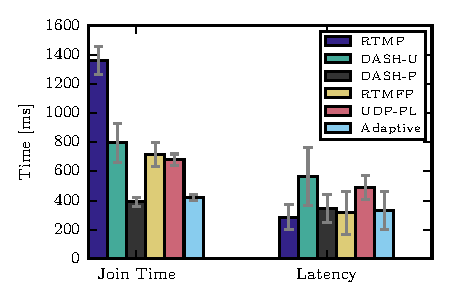
\includegraphics{./gfx/500_MobileUpload/networkAdaptiveComparison}}
\subfloat[]{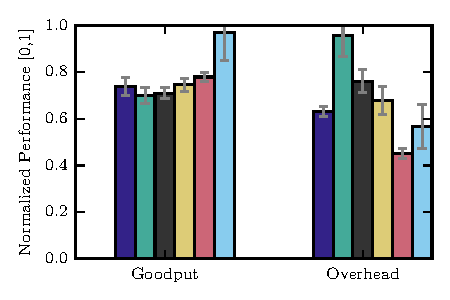
\includegraphics{./gfx/500_MobileUpload/networkAdaptiveComparisonB}}%\\
	\caption[Simulation results on the performance of different MBSs]{Utility and costs of the different MBSs and the adaptation between the protocols. (a) The achieved join time and delay is depicted, whereas in (b) the normalized goodput and the normalized overhead of the protocols are shown.}
	\label{fig:520_SessionAdaptation}
\end{figure}
\subsubsection{"Adaptive"}
The results for using adaptations between protocols are also depicted in Figure~\ref{fig:520_SessionAdaptation}.
Major findings that can be drawn when using an adaptation are a slightly increased overhead and the advantage of always selecting the best protocol available.
\paragraph{Adaptive Video Streaming}
 One of the major advantages of "Adaptive" is the support for adaptive video streaming.
 It affects both the average bit rate and the \ac{stalling} rate positively.
 The average bit rate of the complete video streaming session increases on average by 24.4\%, because "Adaptive" can switch to a higher bit rate representation of a video when the throughput conditions are good.
 At the same time, a low bit rate version of the video may reduce the video quality, but allow a decrease in the average stall time by around 6.2\% to the next best protocol.
 As a result, the \ac{CI} is close to one (0.98) for "Adaptive". 
\paragraph{Advantages of the Protocol Adaptation}
As Figure~\ref{fig:520_SessionAdaptation} shows the adaptive scheme is always close to the best protocol.
Due to its design of switching between existing protocols, the adaptive scheme never significantly outperforms existing schemes. 
In comparison to \ac{RTMP}, adapting protocols generate 3.1\% more overhead, as duplicate messages and coordination overhead are generated.
The adaptations between protocols achieve a similarly low join time as \ac{DASH-P}, but it saves approximately 9.47\% of the overhead.
The additional overhead of the "Adaptive" is rather low in relation to the average video bit rate, i.e., 0.89\% of the average traffic represent protocol overhead.
Only 0.67\% of this overhead represents redundant messages or additional coordination operations.
\paragraph{Switching between Protocols}
In the described scenario, adaptations are invoked every 58 seconds. 
The average adaptation time is related to the new protocol after the adaptation, and it mainly consists of the join time.
Thus, whereas a switch to \ac{DASH-P} is possible with a negligible delay, the remaining upload protocols need up to 1.4 seconds for establishing a streaming session.
By design of the application, an adaptation between two upload protocols is done by running them in parallel until a switch can be achieved.
\subsubsection{In Situ Streaming}
The focus of this study lies in the remote streaming case for analyzing the potential of different \ac{MBS}s and the adaptation between them.
All the existing models assume a constantly available device acting as the receiving server, where persistent, mostly \ac{TCP}-based connections are established.
This is contrary to the proposed "in situ streaming" in which spontaneous connections to any device in the vicinity can be established.
Due to device mobility and the lack of infrastructure-based networks, frequent bandwidth changes and connection losses can occur.
Here, \ac{UDP}-based protocols such as \ac{RTMFP} are advantageous.
The discussed protocols cannot cope with the lack of central coordination, communication range loss, and an increased device mobility.
\subsection{Findings of the Study}
The central findings of the conducted study will be summarized, as they are essential to understand the design of \ac{LiViU} discussed in the next section.
It is the aim that \ac{LiViU} supports varying scenarios, i.e., remote, in-situ, and hybrid streaming, as well as changing application requirements. 

\ac{UDP} offers superior performance in error-free conditions, but even the standardized and widely used protocols such as \ac{RTMFP} neglect the advantages and show similar issues as the \ac{TCP}-based protocols, e.g., a slow join time.
A novel \ac{MBS} should leverage the advantages offered by \ac{UDP}.

The push-based \ac{UDP} transmission has more superior performance in the concurrent streaming scenario for goodput.
\ac{RTMFP} requires an in-order sending of messages, which are all acknowledged.
This adds overhead and leads to additional delay if a message is lost. 
As soon as the sender does not receive an acknowledgment, the message is sent again. 
In general, the scheduling mode (either push- or pull-based) has a higher influence on the performance metrics than the transport layer protocol (either \ac{UDP} or \ac{TCP}).
Pull-based protocols are suitable when a centrally executed application requires specific chunks of video streams.
Switching between these scheduling mechanisms shows promising potential. 
To conclude the findings for scheduling, different schemes promise to support varying application requirements, as, e.g., pull-based delivery allows a central coordination by a server, whereas push-based delivery supports low-delay streaming.

Two other findings are made that address the joining procedure and content adaptation usage. The joining procedure has a major influence on the liveliness of a video stream. It varies significantly between the protocols and should be designed in a manner to quickly distribute the video stream and avoid long-term joining procedures.
Also, none of the protocols leverages adaptation of the video on the mobile device; thus, they cannot cope with changing upload conditions as efficiently as "Adaptive".
The simulative evaluation has shown how beneficial adaptive video streaming is.

For the in situ streaming, the number of connections per device is higher, as a single device has to stream to all receivers instantly.
Even though it has not been validated in the simulations, the challenges are obvious, and it is clear that no discussed protocol offers solutions.